\clearpage

\begin{usecase}
  \addheading{Use-Case Description}
  \addsingletwocolumnrow{Name}{oeGetAlertSet}
  \addsingletwocolumnrow{Scope}{System}
  \addsingletwocolumnrow{Altitude}{subfunction}
  
  \addrowheading{Parameters}
  \addnumberedsinglerow{}{\msrcode{AlertStatus:etAlertStatus} � the Alert status.}
  
  \addrowheading{Primary actor(s)}
  \addnumberedsinglerow{}{\msrcode{actCoordinator[active]}}
  
  \addrowheading{Secondary actor(s)}
  \addnumberedsinglerow{}{\msrcode{actDomainExpert[passive]}}
  
  \addrowheading{Goal(s) description}
  \addsinglerow{the \msrcode{actCoordinator}'s goal is to get a list/set of all the Alerts of a certain alert-status.}
  
  \addrowheading{Reuse}
  \addnumberedsinglerow{}{none}

  \addrowheading{Protocol condition(s)}
  \addnumberedsinglerow{}{the \msricrash system has been deployed.}
  \addnumberedsinglerow{}{the \msrcode{actCoordinator} has logged on to the system.}

  \addrowheading{Pre-condition(s)}
  \addnumberedsinglerow{}{none}
  
  \addrowheading{Main post-condition(s)}
  \addnumberedsinglerow{}{the \msrcode{actCoordinator} is now aware of all the Alerts of a specified status.}
  
  
  \addrowheading{Main success steps}
  \addalphanumberedsinglerow{}{the actor \msrcode{actCoordinator} sends the message \msrucname{oeCloseCrisis(crisisID)} to the system.}
  
  \addrowheading{Step Constraints Ordering and Extensions}
  \addnumberedsinglerow{}{none}
  
  \addrowheading{Additional Information}
  \addsinglerow{none}
  
\end{usecase} 

\clearpage

 \clearpage

 \begin{figure}[htbp]
 \begin{center} 
 \scalebox{0.95}{
 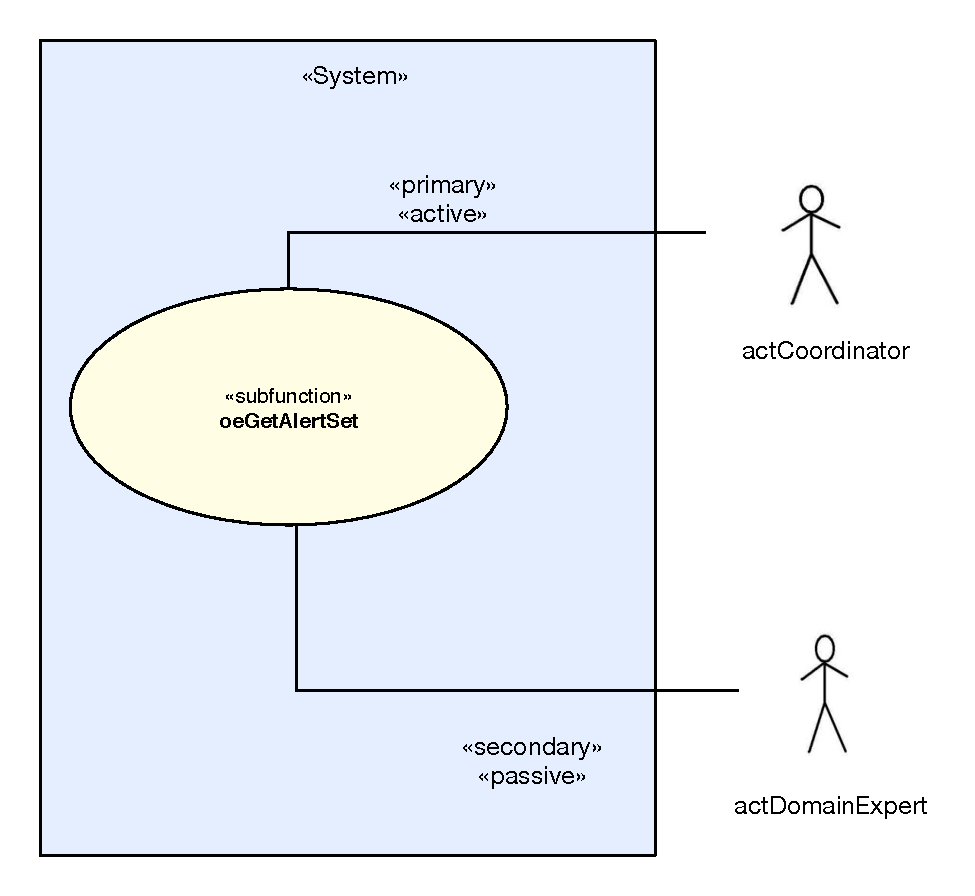
\includegraphics[width=180mm]{./images/oeGetAlertSet.eps}
 \normalsize}
 \end{center}
 \caption[\msricrash Use Case Diagram:  oeGetAlertSet Diagram]{\msricrash Use Case Diagram:  oeGetAlertSet}
 \label{fig:icrash-RE-UCD- oeGetAlertSet}
 \end{figure}
 \vspace{0.5cm}
